%%%%%%%%%%%%%%%%%%%%%%%%%%%%%%%%%%%%%%%%%
% Short Sectioned Assignment
% LaTeX Template
% Version 1.0 (5/5/12)
%
% This template has been downloaded from:
% http://www.LaTeXTemplates.com
%
% Original author:

% Frits Wenneker (http://www.howtotex.com)
%
% License:
% CC BY-NC-SA 3.0 (http://creativecommons.org/licenses/by-nc-sa/3.0/)
%
%%%%%%%%%%%%%%%%%%%%%%%%%%%%%%%%%%%%%%%%%

%----------------------------------------------------------------------------------------
%	PACKAGES AND OTHER DOCUMENT CONFIGURATIONS
%----------------------------------------------------------------------------------------

\documentclass[paper=a4, fontsize=11pt]{scrartcl} % A4 paper and 11pt font size

\usepackage[T1]{fontenc} % Use 8-bit encoding that has 256 glyphs
\usepackage{fourier} % Use the Adobe Utopia font for the document - comment this line to return to the LaTeX default
\usepackage[english]{babel} % English language/hyphenation
\usepackage{amsmath,amsfonts,amsthm} % Math packages

\usepackage{lipsum} % Used for inserting dummy 'Lorem ipsum' text into the template

\usepackage{enumitem}
\usepackage{mathtools}
\DeclarePairedDelimiter\ceil{\lceil}{\rceil}
\DeclarePairedDelimiter\floor{\lfloor}{\rfloor}
\usepackage{graphicx}
\usepackage{subfig}	
\usepackage{listings}
\usepackage{amsmath}
\usepackage{algorithm}
\usepackage[noend]{algpseudocode}
\makeatletter
\def\BState{\State\hskip-\ALG@thistlm}
\makeatother

\usepackage{sectsty} % Allows customizing section commands
\allsectionsfont{\centering \normalfont\scshape} % Make all sections centered, the default font and small caps

\usepackage{fancyhdr} % Custom headers and footers
\pagestyle{fancyplain} % Makes all pages in the document conform to the custom headers and footers
\fancyhead{} % No page header - if you want one, create it in the same way as the footers below
\fancyfoot[L]{} % Empty left footer
\fancyfoot[C]{} % Empty center footer
\fancyfoot[R]{\thepage} % Page numbering for right footer
\renewcommand{\headrulewidth}{0pt} % Remove header underlines
\renewcommand{\footrulewidth}{0pt} % Remove footer underlines
\newcommand{\itab}[1]{\hspace{0em}\rlap{#1}}
\newcommand{\tab}[1]{\hspace{.2\textwidth}\rlap{#1}}

\setlength{\headheight}{13.6pt} % Customize the height of the header

\numberwithin{equation}{section} % Number equations within sections (i.e. 1.1, 1.2, 2.1, 2.2 instead of 1, 2, 3, 4)
\numberwithin{figure}{section} % Number figures within sections (i.e. 1.1, 1.2, 2.1, 2.2 instead of 1, 2, 3, 4)
\numberwithin{table}{section} % Number tables within sections (i.e. 1.1, 1.2, 2.1, 2.2 instead of 1, 2, 3, 4)

\setlength\parindent{0pt} % Removes all indentation from paragraphs - comment this line for an assignment with lots of text

%----------------------------------------------------------------------------------------
%	TITLE SECTION
%----------------------------------------------------------------------------------------

\newcommand{\horrule}[1]{\rule{\linewidth}{#1}} % Create horizontal rule command with 1 argument of height
\title{	
\normalfont \normalsize 
\textsc{University of Toronto, Department of ECE} \\ [25pt] % Your university, school and/or department name(s)
\horrule{0.5pt} \\[0.4cm] % Thin top horizontal rule
\huge ECE1762 - Homework 3 \\ % The assignment title
\horrule{2pt} \\[0.5cm] % Thick bottom horizontal rule
}

\author{Xinyun Lv(1001091178), Yang Wang(1001319227)} % Your name

\date{\normalsize\today} % Today's date or a custom date

\begin{document}

\maketitle % Print the title
\section{Problem I}
\textbf{solution}:\\
According to the description above, this problem could be mapped to a single source Directed acyclic graph(DAG) as follows:
\begin{itemize}
	\item Corridors $\rightarrow$ directed edge
	\item Elevators $\rightarrow$ directed edge
	\item Food Location $\rightarrow$ vertex
	\item Exit Point $\rightarrow$ vertex
	\item Entry Point $\rightarrow$ vertex source
	\item Food Quantity $\rightarrow$ weight on vertex
\end{itemize}

So, the input of this problem is a DAG denoted as $G(V, E)$. And the quantity of food at food location could also be described as the weight on every edge directed to the corresponding food location(vertex). The output should be a path $P$ in $G$ that accumulate the max gain(food) across all paths in $G$ from $S$ to any vertex.

\begin{figure}[h]
\centering
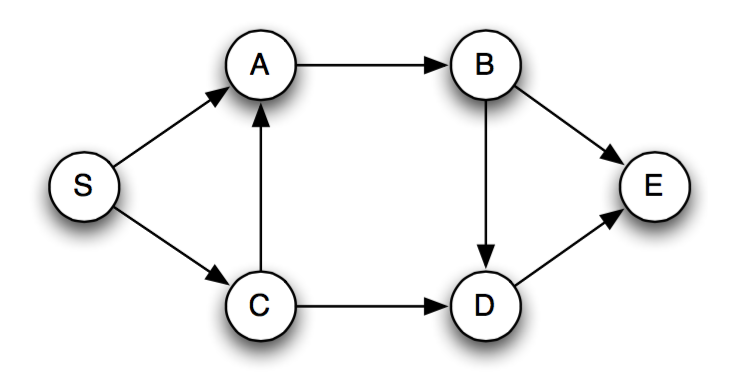
\includegraphics[scale=0.4]{DAG}
\caption{A DAG example mapped from problem}
\label{fig:p1}
\end{figure}

For example, suppose we have a DAG as shown in Figure \ref{fig:p1}. We could traverse the vertices in linearized order from left to right since a DAG can always be topologically sorted or linearized. As shown in Figure \ref{fig:p2}, we the linearized version of the DAG shown in Figure \ref{fig:p1} are then: $\left\{S, C, A, B, D, E\right\}$. 

\begin{figure}[h]
\centering
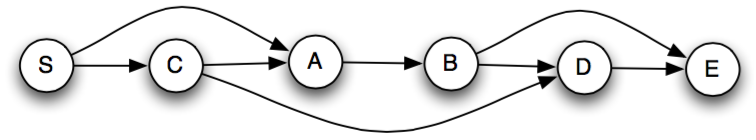
\includegraphics[scale=0.4]{lineardag}
\caption{Linearized version of $G$}
\label{fig:p2}
\end{figure}

The problem equivalent to find the longest path from vertex $S$ to any other vertex. Consider the vertex $D$ in the linearized graph - the only way to get to $D$ from $S$ is through one of its predecessors: $B$ and $C$. That means, to compute the longest path from $S$ to $D$, one must first compute the longest path from $S$ to B (up to the first predecessor), and the longest path from $S$ to $C$ (up to the second predecessor). Once we've computed the longest paths from $S$ to these two predecessors, we can compute the longest path to $D$ by taking the larger of these two, and adding $w(D)$(food quantity in $D$). If $dist(v)$ is the longest distance from $S$ to vertex $v$, and $\alpha(v)$ is the actual path, then we can write the following recurrence for $dist(D)$:

$$ dist(D) = max\left\{ dist(B) + w(D), dist(C) + w(D) \right\} $$

Note the subproblems here: $dist(B)$ and $dist(C)$, both of which are “smaller” than $dist(D)$. Similarly, we can write the recurrences for $dist(B)$ and $dist(C)$ in terms of its subproblems:

$$ dist(B) = dist(A) + w(B) $$
$$ dist(C) = dist(S) + w(A) $$

For the source vertex $S$, we set:

$$ dist(S) = w(S) $$
$$ \alpha(S = \left\{ S \right\} $$

We are now ready to write the recurrence for the longest path from $S$ to any other vertex $v$ in $G$, which involves first computing the longest paths to all of $v$'s predecessors from $S$ (these are the subproblems).

$$ dist(v) = max_{(u, v) \in E}{dist(u) + w(v)} $$

And, we can compute this bottom-up for each vertex $v \in V$ taken in a linearized order. The final algorithm is shown below:\\

LONGEST-PATH($G$)\\
Input: Weighted DAG $G$\\
Output: Largest path cost in $G$\\
Topologically sort $G$\\
\textbf{for} each vertex $v \in V$ in linearized order\\
\hspace*{0.6cm} \textbf{do}:\\
\hspace*{0.6cm} dist($v$) $\gets$ $\text{max}_{(u, v) \in E}\left\{ \text{dist}(u) + w(v) \right\}$\\
\hspace*{0.6cm} $\alpha(v) \gets \text{max}_{(u, v) \in E}\left\{ \alpha(u) \cup v \right\}$\\
\textbf{return} $\text{max}_{v \in V} \left\{ \text{dist}(v) \right\}$\\

The time complexity is obvious $O(\mid V \mid + \mid E \mid)$.


\section{Problem I}
\textbf{solution}:\\
\begin{enumerate}
	\item \textbf{proof:} \\
	Without loss of generality, suppose that $I_m > I_t$ are two elements in $\langle I_1, I_2, ..., I_k \rangle$ where $1 \leq m \geq k$, $ 1 \leq t \leq k $ and $m \neq t$. Suppose that Greedy-Schedule determines order $I_m \succ I_t$ on $I$. Greedy-Schedule determines an order $I_m \prec I_t$ on $I'$.\\

	From definition of order restriction, for $I_m, I_t \in I$ and $I_m, I_t \in I'$. $I_m$ precedes $I_t$ \textbf{iff} it also determines an order on $I'$ where $I_m$ precedes $I_t$ yielding a contradiction to the assumption that $I_m \succ I_t$ on $I$, $I_m \prec I_t$ on $I'$. The opposite direction is the same. Thus, Greedy-Schedule determines an order $I_1 \succ I_2 \succ ... \succ I_k$ on $I$ if Greedy-Schedule determines an order $I_1 \succ I_2 \succ ... \succ I_k$ on $I'$. 
	\item \textbf{proof:}\\
	we first prove if (a), (b) and (c) happens $\Rightarrow$ Greedy-Schedule is not correct.\\

	If we use algorithm First Starting Time First which means we choose interval in $I$ with the earliest start time. Let interval $I[a], I[b], I[c] \in I $ where $s_a < s_b < s_c$ and $f_c < f_a$ and $f_b < s_c$. For these three intervals, they meet (a), (b), (c) as shown in the figure.\\

	If we choose interval in $I$ with the earliest start time, then we will choose $I_a$ instead of $I_b$ and $I_c$. For optimal schedule, we should choose $I_b$ and $I_c$ instead of $I_a$ since we could schedule more intervals within the same time slot. Thus, Greedy-Schedule is not optimal. \\

	Greedy-Schedule is not correct $\Rightarrow$ (a), (b), (c) happens. \\

	If Greedy-Schedule is not optimal, which means it will choose less intervals compare with the optimal set. If Greedy-Schedule $GS$ is not optimal and $I_a, I_b, I_c \in I$. As $GS$ is not optimal we can assume that $GS$ picked $I_a$ instead of $I_b, I_c$. But for the optimal schedule set($OS$), it choose $I_b$ and $I_c$ instead of $I_a$. Which means that $I_a$ should overlap with $I_b$ and $I_c$. So they could not be chosen at the same time. Which meets the situation (a). As $I_b$ and $I_c$ could be chosen together which implies that $I_b$ and $I_c$ does not overlap with each other. So it also meets situation (b). As in $GS$, $I_a$ is chosen first, so we could not choose $I_b$ and $I_c$. Which implies that on input I Greedy-Schedule determines an ordering $O$ where $I[a]$ comes before $I[b]$ and $I[c]$, so situation(c) also happens. 

	\item \textbf{proof:} \\
	According to the conclusion in question (2), we know that Greedy-Schedule is correct iff (a), (b), (c) not happens. So to prove LSTF is correct, is equivalent to prove (a), (b) and (c) cannot happen. \\

	Suppose that for LSTF, (a), (b), (c) happens. For $I_a, I_b, I_c \in I$. We let $s_i, f_i$ be the start time and finish time of interval $I_i$. If (a) is true, here without loss of generality, we let $I_b$ precedes $I_c$,  then $s_a < f_b$ (1) and $ s_c < f_a $. If (b) is true. $f_b < s_c$ (2). From (1) and (2) we know that $s_a < f_b < s_c$ (3). If (c) is true, according to the rules of LSTF, as $I_a$ precedes $I_b, I_c$, $s_a > s_b > s_c$ which contradict (3). So, for LSTF (a), (b), (c) cannot happen together. Thus LSTF is correct. 
\end{enumerate}
\section{Problem III}
\section{Problem IV}
\section{Problem V}
\end{document}